\chapter{Introduction}
\label{chapter:introduction}

%\minitoc
\chapterwithfigures{\nameref*{chapter:introduction}}
%\chapterwithtables{\nameref*{chapter:introduction}}

\ifthenelse{\boolean{skipIntro}}{\endinput}{}

% \todo{1 + 2 + 3 doit etre fini pour mercredi matin !!}\\
\todo{le 15 je mets un message aux repporteurs en disant que j'aurai une version finale le 1 aout, 15 j en retard}\\
\todo{quand ils valident le jury alors faut que je valide sur adum}\\
% efficient image editing w/pretrained generative models 
% today; big models are available to use w/o having to re-train 
% state of the art 

% context IA / machine learning / CV 
% contributions -> edition ; what is the problem that i announced 
% exploit recent generative models 

% \epigraph{In a world once ruled by human hand\\
% Now machines have claimed the land\\
% Artificial intelligence reigns supreme\\
% Their circuits calculating the grand scheme.}{\textit{Automatically generated by ChatGPT}}

\todo{intro - intro contrib tres coarse; comme related work mais tres coarse. environ 5 pages}

\emph{The camera doesn't lie}. We like to think of photographs as a perfect 
reflection of the Truth. They allow us to understand the present or truly 
glance back in time into history. 
Written documents can be easily altered, but surely not brilliantly complex photographs. 
Alas, the first edited photo in 1860\todo{cite} only shortly followed 
 the invention of photography itself in the 1820s. 
 During the 1920s, Stalin's regime led a massive photo 
 doctoration campaign, where 
opponents were quite literally (and realistically) erased from the history
 books 
through manual techniques like 
rephotographing photographs and chemical processing. \todo{cite} Digital 
image 
editing appeared in the 1980's, with PhotoShop emerging and quickly dominating 
the industry. Technologies such as color enhancement, colorization, and composition 
allowed photographers to create just about anything they imagined, provided they 
spend enough time. \todo{how long} In the early 2010s, deep convolutional neural networks started dominating tasks like image classification \todo{cite},
and early works in Generative Networks appeared shortly after. However, it was not until 
the early 2020s that truly realistic generation was made possible, and fast and intuitive 
photo editing applications were released \todo{cite}. Today, \emph{semantic image editing}, 
where high-level image characteristics are easily modified, is finally possible (albeit not 
yet perfect). An 
image edit which may have taken hours just a few years ago can now be achieved in a matter of seconds. This thesis, started in 2020, had the unique opportunity to benefit from 
the recent groundbreaking advances in \emph{generative AI}. Indeed, our work
 followed and contributed to the recent trends in 
photo editing which allowed intuitive and semantic image editing. 



% It's rare for two simple letters - AI - to evoke such diverse and strong emotions, ranging from wonder and excitement to bewilderment,
% to fear and distress, and to flat-out disappointment. For a typical member of our modern Western society,  \ac{AI} is used
% all day, every day. Our music and movies are recommended to us by \ac{AI} recommender-systems \citep{toscher2009netflixprize}, 
% our driving directions are calculated by \ac{AI}\note{what is the technology for this ? cite}, our headphones use \ac{AI} 
% noise-cancelling technology \citep{noise_cancelling}, and we can ask \ac{AI} systems like "Siri" any questions using only our voice. 

Artificial Intelligence refers to the development of computer systems which are able to perform tasks which typically require 
human-intelligence. The term \ac{AI} is ambiguous and constantly evolving - what are the tasks which "typically require human-intelligence"? 
Optical character recognition, which converts printed texts into digital files, has become so mundane that it is typically not 
considered to be \ac{AI}. For simplicity's sake, the \ac{AI} that we refer to in our work can be more precicely defined as 
\ac{ML}, which consists in (1) designing a parameterized mathematical model, a \ac{NN} $f_\theta$ as well as a loss function and 
(2) developing algorithms to calculate the parameters $\theta$ of the \ac{NN} which minimize the loss 
function using real-world data as the "ground-truth". In particular, complex and "deep" functions, referred to as 
\ac{DNN}, are defined using upwards of 175 billion learnable parameters \citep{gpt3}! This branch of \ac{AI}, \ac{DL}, 
has achieved remarkable results in recent years, which have fueled today's research trends of making bigger models and training 
with more data. In this work, we more specifically delve into the realm of \ac{CV}, which focuses on the understanding and manipulation of 
numerical images. Indeed, numerical images can be easily
represented to a computer in the form of RGB matrices.

%\ac{AI} research was born in the 1950's, where computers were learning to play checkers, solving algebra problems, 
% and speaking English. \note{continue with a bit of history}.

Throughout recent history, society at large went from waves of excitement and fear to sheer disappointment about the prospects 
of \ac{AI}. \ac{AI} confonted people with the uncomfortable question, "what does it mean to be human?". As \ac{AI} started beating 
humans in checkers\note{cite}, then chess\note{cite}, and more recently Go\note{cite}, humans reluctantly accepted that computers are 
superior in developing long-term strategy in games with simple rules and rewards. Likewise, language generation and translation, previously 
thought to be too complicated and nuanced for computers to understand, has achieved human-like capacities in recent years. Of course,
society has always clinged to the last untouchable area of unique human-ness - creativity. Machines can coldly and robotically 
calculate game movements and translate language, but machines couldn't possibly have the creativity to create images which match 
the genius of Leonardo da Vinci or Picasso. However, this again proved to be false when a computer-generated image won an artwork
competition \note{cite} in 2022 using the latest generative models. 

This thesis will explore this subfield of Generative AI \note{cite}, and in particular, image editing with \ac{DNN}s.


As we will come to see, editing real images with AI is a unique case where the "artificial" meets "human". 
Indeed, while a fake image 
which is entirely generated by an AI system is trained to be harmonious by the model, an edited image
requires a generation which is not only realistic but also faithful to the original image. This 
tradeoff between \emph{editing success} and \emph{fidelity to the original image} is a recurrent theme which we will see throughout 
our thesis, both to build our methods as well as evaluate them. We tackle several different families of editing operations (attribute editing, 
text-guided editing, and inpainting) and leverage different generative models to accomplish our task. 


\section{PhD Thesis Context}

\paragraph{Meero}
Created in 2014, Meero is a French startup which specializes in digital image processing using \ac{AI}. Meero made history in 2019 when 
it raised a record-breaking \$230 million, becoming one of France's only "unicorns". Meero enhances real-world world images from markets
ranging from real-estate to food photography to e-commerce. Meero proposes technology such as background-removal, color-enhancement, object 
removal and super-resolution. The majority for these image-manipulation algorithms relies on research in \ac{DL}.
It is important to note that there is often a disparity between the results proposed by state-of-the-art research for \note{constructed}
datsets and the expected image quality Meero's clients have. Firstly, research in the field often works with ``small" images 
(ImageNet\note{cite}, for example, uses 256x256 resolution). Meero's clients often work with images of upwards of 5000x5000 resolution, 
which brings challenges for deep learning applications.  Moreover, generated images in research papers quite often have 
visible artifacts, which is acceptable in the context of research but inconcevable to present to clients expecting a beautiful 
image. A goal of this thesis is to explore image editing specifically with the goal of achieving aesthetic images.

However, there
is quite often a disparity between quality of images from state-of-the-art research in the field and the picture-perfect quality that 
Meero's clients expect in the real world. The goal of this thesis is to bridge this gap. 

\begin{figure}[tb]
      \begin{center}
          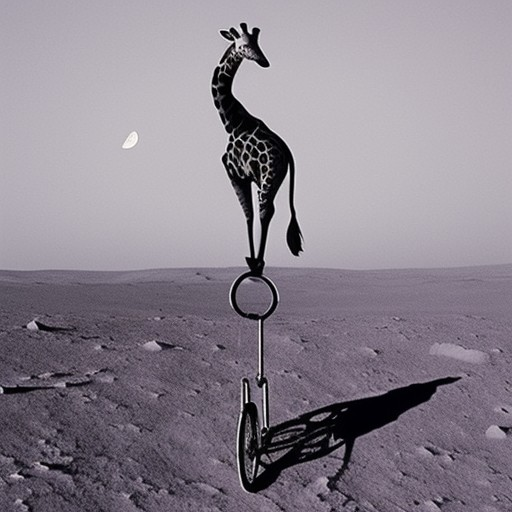
\includegraphics[width=0.5\linewidth]{images/intro/giraffe.png}
      \end{center}
      \caption{Using Stable Diffusion\note{cite} to generate a photo of "a giraffe riding a unicycle on the moon"}
      \label{fig:diffusion_example}
  \end{figure}


\paragraph{Image Generation}
Image generation has seen phenomenal and almost unbelievable progress in recent years, mainly due to improvements in model architecture. 
In 2013, the Variational Auto-Encoder (\ac{VAE}) \note{cite} allowed blurry, low-quality results of images in a particular domain. In 2014,
\ac{GAN}s were introduced, which Yann LeCun, the \ac{DL} pioneer, described as “the most interesting idea 
 in the last 10 years in Machine Learning”. Indeed, the "generator" was trained not alone, but in unison with another network, the "discriminator",
 both trained "adversarilly" (their respective objectives are opposing). The \ac{GAN} frenzy lasted until the start of the 2020's, and for the
  first time  allowed truly realistic generations of images in restricted domains, particularly faces. Indeed, the popular webiste
   \emph{thispersondoesnotexist.com} displayed the uncannily realistic face generations using StyleGan\note{cite!}. However, \ac{GAN}s struggled with 
   larger and more diverse domains, leaving room for other architectures, like Vision Transformers \ac{ViT, VQGAN}s to fill the gap. Only recently,
   remarkable progress was made with Diffusion Models \note{cite}. These models, as we will later see, have a simple loss function and allow stable training.
   As Diffusion Models quickly made their way to becoming state-of-the-art for various datasets, particularly ImageNet\note{cite}, researchers
   started to scale up the models and train them on massive billion element text-image datasets. The past few years have welcomed
   a true revolution in Image Generation, allowing generation of images which are not only realistic, but also of unprecedented diversity.
   Indeed, a completely imaginary and absurd prompt such as "a giraffe riding a unicycle on the moon" actually produces a  plausible 
   output image, as shown in \ref{fig:diffusion_example}.

   

% challenge / contributions
/todo{challenges !! talk about challenges}
/todo{mets les publis a chaque fois}

\note{cite} first proposed ma
- VAE 

\paragraph{Image Editing}
Talk about photoshop; semantic editing applications; etc.


\todo{why do people today have a problem with it; history of ethical concerns, "creativity" one of the last
 branches getting eated by AI}


 

In this thesis, we studied this "creativity" branch of AI. We strived to use AI deep learning systems to edit real images. 

\paragraph{Leveraging pre-trained models}
\note{write about how using pre-trained models is very useful because blablabla}





% In this thesis introduction, using layman terms, we describe Artificial Intelligence, and,
% in particular, one of its instances: Deep Learning. Then, we lay out the challenges of this
% thesis and our contributions.

% %\section{Artificial Intelligence}

% \textbf{The idea of thinking machines} began in the previous century, from Karel Çapek's invention
% of the "\textit{robot}" to the 1956's Dartmouth workshop passing by Turing \& von Neumann's
% reflections. Despite suffering from multiple "AI winters" filled with disappointments and
% criticisms, Turing's prediction on the rising importance of \ac{AI} proved to be right as the first
% and the second decades of the XXI century saw the advent of respectively \acf{ML}
% \citep{bishop2006prml} and \acf{DL} \citep{goodfellow2016deeplearningbook}, two major subfields of
% \ac{AI}, related to statistical learning theories.

% Providing \textbf{a definition of \ac{AI}} is difficult, but its foremost domains, \ac{ML} and
% \ac{DL}, can be defined as statistical algorithms that can improve automatically through experience
% and the use of data. These methods are already ubiquitous: speech recognition enabling us to control
% devices remotely \citep{amodei2016deepspeech2}, recommender systems proposing movies according to
% our taste \citep{toscher2009netflixprize}, automatic translation \citep{vaswani2017transformer},
% face recognition \citep{schroff2015facenet}, autonomous driving \citep{sun2020waymodataset}, \etc.
% Less known but still useful applications comprise accelerated physics simulation
% \citep{breen2020threebody}, protein folding prediction \citep{jumper2021alphafold}, molecule
% toxicity estimation \citep{nih2019toxchallenge}, data center cooling
% system \citep{evans2016datacentercooling}, control of the magnetic coils of a nuclear fusion reactor
% \citep{degrave2022nuclearreactor}, \etc.

% \ac{AI} is increasingly more important in our daily lives with some applications raising
% \textbf{ethical concerns}: face recognition biased towards some populations
% \citep{grother2019facerecoethic}, loan grants \citep{anglekar2021loangrantml}, medical diagnosis
% \citep{lazzazabal2020medicalbias}, justice advice \citep{russel2020justicefairness}, biased chatbots
% \citep{sheng2019lmbias}, \etc. Therefore, we must pay a particular interest in the potential impact
% of this new technology. Towards this goal, people from diverse backgrounds must participate in the
% creation of such technology, and standardization bodies \citep{tommasi2021fairness} should advise
% what types of \ac{AI} systems can be used in which scenarios \citep{gebru2019aiethichandbook}.

% \section{PhD Thesis Context}

% I now contextualize my thesis with relation to my sponsor, how it influenced our research, and what
% challenges we have aimed to tackle.

% \paragraph{Heuritech} This thesis was sponsored by the Parisian startup
% Heuritech\footnote{\url{https://heuritech.com}} as a \textit{CIFRE PhD}. The company analyzes social
% networks such as Instagram and Weibo, recognizes the clothes in pictures, estimates
% volumes of fine-grained types of garments, and finally forecasts future trends. The company's
% \acf{CV} models must recognize an ever-growing number of entities from features (\eg knitted, blue
% color, short cut) to brand models (\eg Nike Air Max, Adidas Stan Smith, Puma Suede). This
% requirement leads to two problems: \textbf{(1)} the time spent to re-train a model is growing
% linearly, and \textbf{(2)} learning a new entity can incur a performance loss on previously learned
% entities.

% \paragraph{Continual Learning} is a field that emerged in the 1990s but saw renewed interest only
% very recently around the second half of the 2010s. The goal is to deal with datasets that evolve
% through time. This evolution can take many forms, including adding new entities to predict in a
% classification task (\eg learning sneaker brands, then high-heel brands) or adding samples from new
% sources (\eg commercial photoshoot then images from social media). Unfortunately, current
% State-of-the-Art models struggle to learn continually from new data without losing performance on
% previously seen data. This loss is so critical that the literature nicknamed it ``\textit{catastrophic
%       forgetting}'' \citep{robins1995catastrophicforgetting,french1999catastrophicforgetting}. Multiple
% methods can reduce this forgetting, including rehearsal and constraints. Rehearsal involves
% reviewing previously learned knowledge, as a human student would \textit{rehearse} the last
% semester's course. However, this rehearsal is often limited in order to reduce computational cost
% and because past data may not always be available for a variety of reasons, including privacy. On
% the other hand, constraints enforce the model to keep a similar \textit{behavior} as it learns new
% concepts, but defining the optimal constraint is not trivial.

% \section{Contributions}

% This PhD thesis is structured around solving catastrophic forgetting in continual settings. We
% considered various specific situations and approaches declined in several chapters:

% \begin{itemize}
%       \item \autoref{chapter:regularization}: \nameref{chapter:regularization}\\
%             We first propose strategies to tackle catastrophic forgetting in deep neural neworks in
%             the context of the image classification. Our main goal is to constrain the evolution of the
%             network parameters during the continual training to be relatively rigid while also
%             avoiding completely freezing the network. The work in this chapter has led to two
%             conference publications:
%             \begin{itemize}
%                   \item \fullcite{douillard2020podnet}
%                   \item \fullcite{douillard2020ghost}
%             \end{itemize}

%       \item \autoref{chapter:segmentation}: \nameref{chapter:segmentation}\\
%             Then, we extend our focus to the task of semantic segmentation. We show that this
%             context brings new challenges, and we propose multiple complementary approaches to tackle
%             them. The work in this chapter has led to one conference publication and one submission
%             to a journal:
%             \begin{itemize}
%                   \item \fullcite{douillard2020plop}
%                   \item \fullcite{douillard2021objectrehearsal}
%             \end{itemize}

%       \item \autoref{chapter:dynamic}: \nameref{chapter:dynamic}\\
%             Finally, in our last chapter, we consider the impact of the neural network architecture
%             for continual learning and in particular propose using the recent Transformer. The work
%             in this chapter has led to a conference publication:
%             \begin{itemize}
%                   \item \fullcite{douillard2021dytox}
%             \end{itemize}
% \end{itemize}

